\documentclass[13pt, a4paper, twoside]{mwart}
\usepackage[a4paper]{geometry}
\geometry{left=3cm}
\geometry{right=1.5cm}
\geometry{top=2cm}
\geometry{bottom=1.5cm}
\usepackage[pdftex]{graphicx}
\usepackage{float}
\graphicspath{{img/}}

\usepackage[utf8]{inputenc}
\usepackage{polski}
\usepackage[polish]{babel}
\usepackage{tabularx}
\usepackage{datetime}
\usepackage{listings}
\lstset{basicstyle=\footnotesize}

\newcommand{\coursename}{Modelowanie i Analiza Systemów}
\newcommand{\labnumber}{3}
\newcommand{\labname}{Dyskretna transformata Z w VHDL AMS}
\newcommand{\studentname}{Maciej Stanek}
\newcommand{\studentnumber}{122352}
\newdate{labdate}{10}{5}{2018}
\newdate{labreportdate}{17}{5}{2018}

\usepackage{fancyhdr}
\pagestyle{fancy}
\fancyhead[RO,LE]{\thepage}
\fancyhead[LO]{\textbf{LAB\#\labnumber} \labname}
\fancyhead[RE]{\coursename}
\fancyfoot{}

\usepackage{xcolor}
\usepackage{framed}
\colorlet{shadecolor}{gray!10}
\newcounter{taskcounter}
\newcommand{\task}[1]{
  \stepcounter{taskcounter}
  \vspace{0.2cm}
  \begin{shaded}
    \noindent\textbf{Zadanie \thetaskcounter:} \textit{#1}%
  \end{shaded}
  \vspace{0.2cm}}

\renewcommand{\labelitemi}{$\bullet$}

\begin{document}

\begin{center}
  \textbf{\LARGE{Sprawozdanie z laboratorium}}
\end{center}

\noindent
\begin{tabularx}{\linewidth}{rX}
  \textbf{Przedmiot} & \coursename \\
  \textbf{Temat laboratorium} & \labname \\
  \textbf{Numer laboratorium} & \labnumber \\
  \textbf{Imię i nazwisko} & \studentname \\
  \textbf{Numer indeksu} & \studentnumber \\
  \textbf{Data wykonania} & \displaydate{labdate} \\
  \textbf{Data sprawozdania} & \displaydate{labreportdate} \\
\end{tabularx}

\vspace{0.3cm}
\noindent\hrulefill

%%%%%%%%%%%%%%%%%%%%%%%%%%%%%%%%%%%%%%%%%%%%%%%%%%%%%%%%%%%%%%%%%%%%%%%%%%%%%%%

\task{Układ sample\&hold ma próbkować napięciowy sygnał wejściowy podawany na terminal input. Próbkowanie ma następować przy narastającym zboczu zegara \texttt{clk}.}

\lstinputlisting[
  language=VHDL,
  caption={Sample\&hold.}
  ]{../122352/hdl/sample_hold.vhd}

\begin{figure}[H]
	\centering
	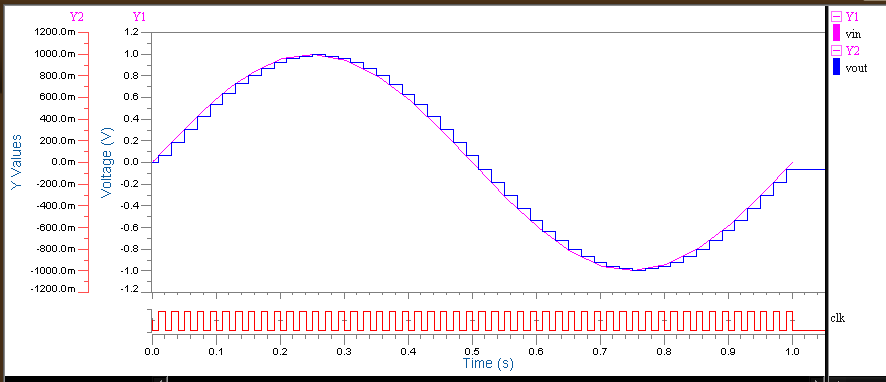
\includegraphics[width=0.6\linewidth]{inv/sample_and_hold.png}
  \caption{Działanie układu sample\&hold.}
\end{figure}

\begin{figure}[H]
	\centering
	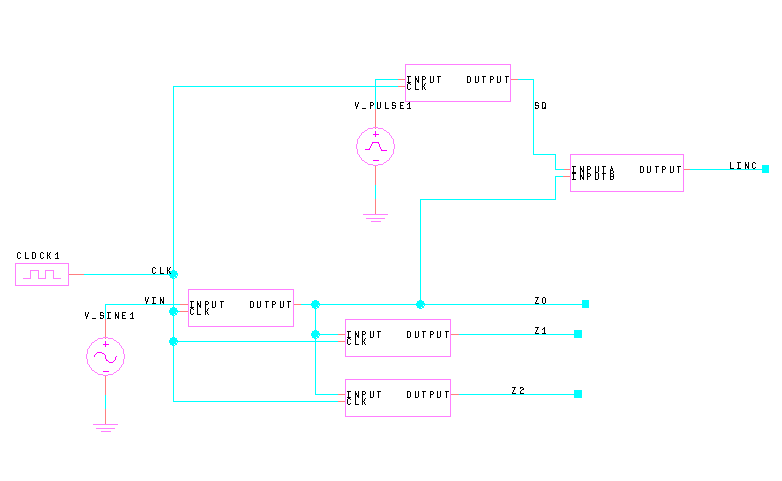
\includegraphics[width=0.6\linewidth]{inv/test_linearcombination.png}
  \caption{Układ testujący blok kombinacji liniowej, układ sample\&hold oraz układy opóźniające.}
\end{figure}

\task{Układ opóźniający ma dwa porty wejściowe: sygnał zegarowy (std\_logic) oraz sygnał wejściowy (real). Na wyjściu sygnał ma pojawić się z n-krotnym opóźnieniem. Opóźnienie zdefiniowane jest w formie parametru generic.}

\lstinputlisting[
  language=VHDL,
  caption={Układ opóźniający $Z^{-n}$.}
  ]{../122352/hdl/zdelay.vhd}

\begin{figure}[H]
	\centering
	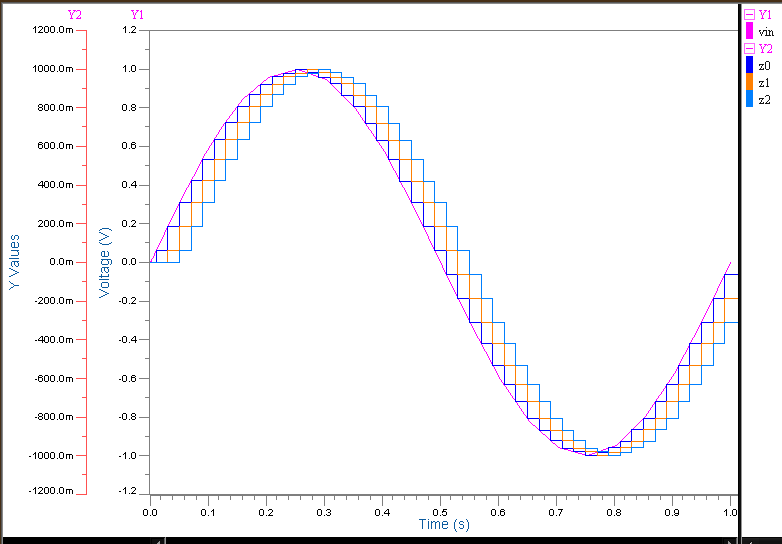
\includegraphics[width=0.6\linewidth]{inv/zdelay.png}
  \caption{Działanie układu opóźniającego.}
\end{figure}

\task{Układ kombinacji liniowej na wejściu ma dwa sygnały typu real i sumuje je z odpowiednimi wagami (kombinacja liniowa). Współczynniki określone w postaci parametrów generic. Układ nie wymaga sygnału synchronizującego zegara. Zaprojektuj architekturę układu w sposób asynchroniczny.}

\lstinputlisting[
  language=VHDL,
  caption={Układ kombinacji liniowej.}
  ]{../122352/hdl/linearcombination.vhd}

\begin{figure}[H]
	\centering
	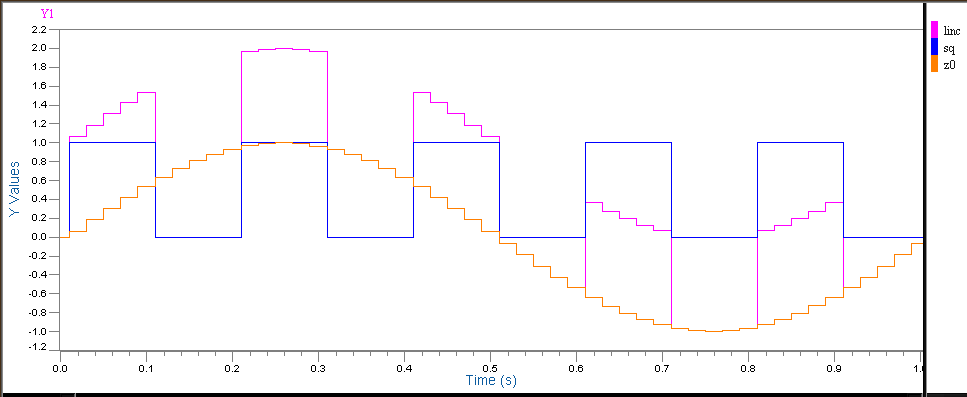
\includegraphics[width=0.6\linewidth]{inv/linearcombination.png}
  \caption{Działanie układu kombinacji liniowej.}
\end{figure}

\task{Zaimplementuj układy integratorów według wyznaczonych na laboratorium schematów blokowych. Do ich implementacji należy wykorzystać wyłącznie układy kombinacji liniowej i opóźniające. Porty wejściowe integratora to sygnał typu real oraz sygnał zegarowy typu std\_logic.}

Implementacji integratorów dokonano behawioralnie, bez wykorzystania gotowych bloków opóźnień.

\lstinputlisting[
  language=VHDL,
  caption={Backward Euler Integrator.}
  ]{../122352/hdl/backint.vhd}

\lstinputlisting[
  language=VHDL,
  caption={Forward Euler Integrator.}
  ]{../122352/hdl/forwardint.vhd}

\lstinputlisting[
  language=VHDL,
  caption={Bilinear Integrator.}
  ]{../122352/hdl/bilinint.vhd}

\task{Korzystając z układów integratorów z poprzedniego zadania przetestuj i porównaj działanie każdego z układów całkujących. Porównaj odpowiedzi układów na wymuszenia impulsem Kroneckera i skokiem jednostkowym z obliczeniami z laboratorium. Wykorzystaj dany układ test--bench do przetestowania układu.}

Zaprojektowane układy zachowują się tak samo, jak układy wzorcowe zaprezentowane na przykładowych wykresach odpowiedzi skokowych i impulsowych.

\begin{figure}[H]
	\centering
	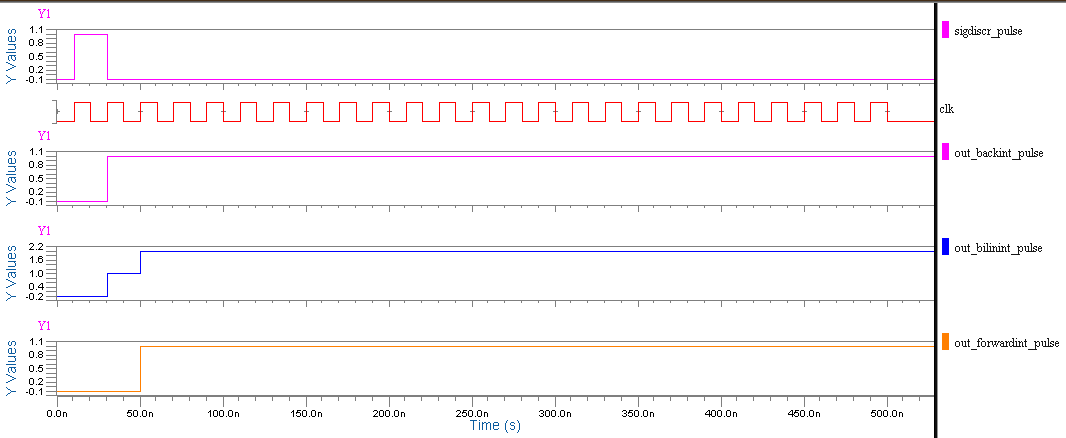
\includegraphics[width=\linewidth]{inv/three_int_pulse.png}
  \caption{Odpowiedź trzech zaprojektowanych układów całkujących na impuls jednostkowy.}
\end{figure}

\begin{figure}[H]
	\centering
	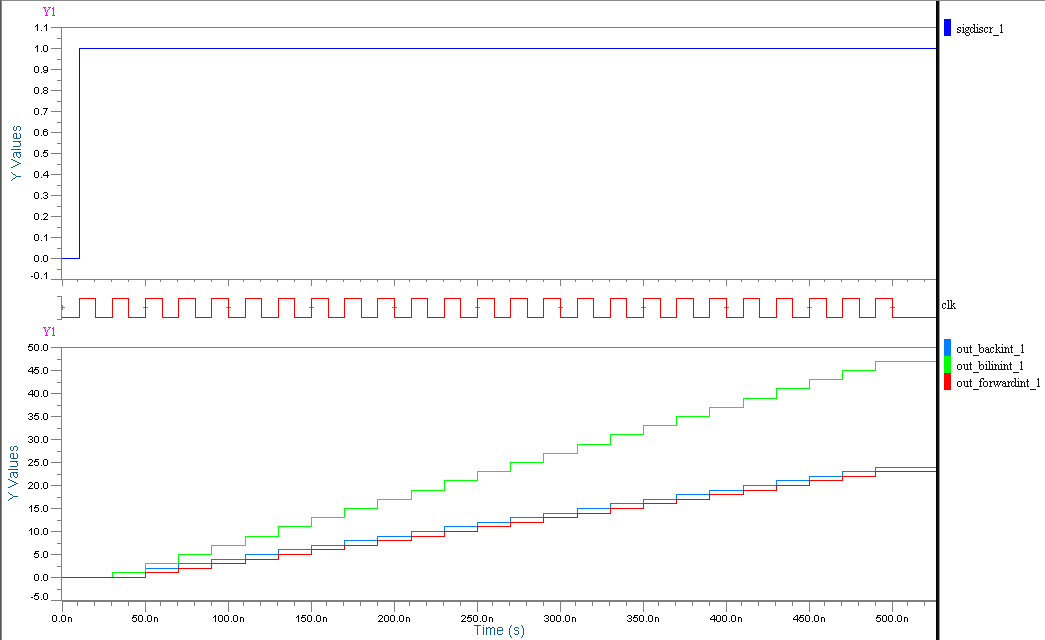
\includegraphics[width=\linewidth]{inv/three_int_step.png}
  \caption{Odpowiedź trzech zaprojektowanych układów całkujących na skok jednostkowy.}
\end{figure}

%%%%%%%%%%%%%%%%%%%%%%%%%%%%%%%%%%%%%%%%%%%%%%%%%%%%%%%%%%%%%%%%%%%%%%%%%%%%%%%

\end{document}
